%% ------------------------------------------------------------------------- %%
\chapter{Experimento}
\label{cap:experimento}


Neste capítulo apresentamos o conjunto de dados, os procedimentos utilizados para treinamento e avaliação do nosso modelo, além das arquiteturas utilizadas para comparação. Descrevemos também o pré-processamento feito no conjunto de dados antes do treinamento. O código-fonte do pré-processamento, bem como o código dos modelos propostos e de comparação, estão disponíveis em um repositório do \Gls{github},  juntamente com o conjunto de dados utilizados, no seguinte endereço: \url{https://github.com/mrezende/concra}.



\section{Conjunto de dados}
\label{sec:conjunto-dados}

Para este estudo, utilizamos parte do conjunto de dados disponibilizados por \cite{yao-2018}. Esse conjunto é formado por $\bm{147.546}$ pares de questões em inglês e trechos de código-fonte em Python e $\bm{119.519}$ em SQL. Estes pares foram coletados do site \Gls{sof} e disponibilizados publicamente através de um repositório no \Gls{github} pelos pesquisadores\footnote{\url{https://github.com/LittleYUYU/StackOverflow-Question-Code-Dataset}}. Uma peculiaridade desses dados em relação aos dados utilizados nos outros trabalhos \cite{iyer-etal-2016-summarizing, Allamanis-bimodal-source-code-natural-language:2015}, é o fato de conter questões do tipo \textit{how-to-do-it}. As respostas para este tipo de questão costumam ser mais diretas e ter apenas um trecho de código-fonte como solução \citep{yao-2018}. Essas questões normalmente expressam as intenções do desenvolvedor, indo ao encontro com a nossa definição da Seção~\ref{sec:code-retrieval-definicao} adotada para o problema de \textit{code retrieval}.

Os dados disponibilizados por \cite{yao-2018} são divididos em 3 (três) subconjuntos distintos. Um subconjunto é formado apenas por questões coletadas do \Gls{sof} que continham apenas um trecho de código-fonte na descrição da resposta. O outro é formado por questões que apresentavam mais de um trecho de código-fonte na descrição. O terceiro é formado por pares de questões e trechos de código-fonte anotados manualmente. A divisão dos subconjuntos podem ser visualizados na Figura~\ref{fig:distinct-subset-python-pair-question-code}.

\begin{figure}[h]
\centering
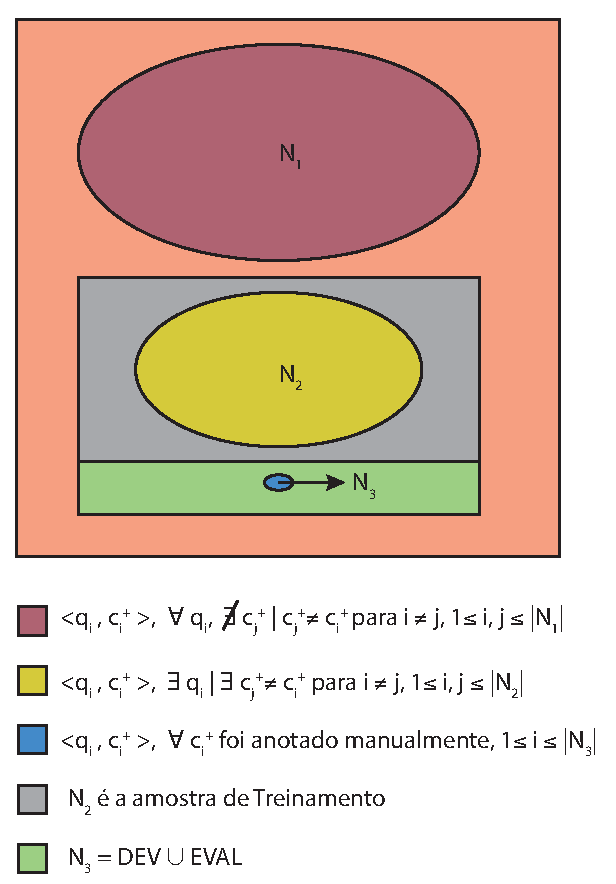
\includegraphics[width=0.6\textwidth]{figuras/cap-experimento/distinct-subsets-yao-sample.pdf}
\caption{Divisão das amostras de pares de questões e trechos de código disponibilizados por \cite{yao-2018}: $N_{1} = \{(q_{i}, c_{i}^{+})\;,\; \forall\; q_{i},\;\nexists\; c_{j}^{+}\; |\; c_{j}^{+} \neq c_{i}^{+}\; \text{para}\; i \neq j,\; 1 \leq i,j \leq |N_{1}| \}$, $N_{2} = \{(q_{i}, c_{i}^{+})\;,\; \exists\; q_{i}\; | \;\exists\; c_{j}^{+} \neq c_{i}^{+}\; \text{para} \; i \neq j,\; 1 \leq i,j \leq |N_{2}| \}$, $N_{3} = \{(q_{i}, c_{i}^{+}),\; \forall\; c_{i}^{+} \text{foi anotado manualmente}, 1 \leq i \leq |N_{3}| \}$. Onde $N_{1} \cap N_{2} \cap N_{3} = \varnothing$, $q_{i} \in \mathbb{Q}$ e $c_{i}^{+},  c_{j}^{+} \in \mathbb{C}$. E $c_{i}^{+}, c_{j}^{+}$ são respostas anotadas como corretas. $\mathbb{Q}$ e $\mathbb{C}$ representam o conjunto de questões e trechos de código respectivamente.} 
\label{fig:distinct-subset-python-pair-question-code}
\end{figure}

Nos casos em que há mais de um trecho de código-fonte na descrição da resposta, um trecho de código não é necessariamente uma solução para a pergunta. No exemplo a seguir, os trechos \emph{T2} e \emph{T4} não são soluções para a questão. O trecho \emph{T2} apenas inicializa um array e o trecho \emph{T4} mostra a saída do comando \textit{print} para o vetor já convertido\footnote{Site: \url{https://stackoverflow.com/questions/34349762/convert-2d-numpy-array-to-string} Esta questão apresenta 6 trechos de código-fonte, mas para melhor visualização, optamos por colocar apenas 4 trechos em nosso exemplo\label{foot:exemplo-stackoverflow-mais-de-um-trecho}}.



\begin{tcolorbox}[colframe=orange!75!black,colback=gray!15!white,fonttitle=\bfseries,adjusted title=\large{Título da questão: convert 2d numpy array to string}~\ref{foot:exemplo-stackoverflow-mais-de-um-trecho}]
\begin{mypythongreen}{Trecho T1: A one-liner will do:}
b = '\n'.join('\t'.join('%0.3f' %x for x in y) for y in a)
\end{mypythongreen}

\begin{mypythonred}{Trecho T2: Using a simpler example:}
>>> a = np.arange(25, dtype=float).reshape(5, 5)
>>> a
array([[  0.,   1.,   2.,   3.,   4.],
       [  5.,   6.,   7.,   8.,   9.],
       [ 10.,  11.,  12.,  13.,  14.],
       [ 15.,  16.,  17.,  18.,  19.],
       [ 20.,  21.,  22.,  23.,  24.]])
\end{mypythonred}
\begin{mypythongreen}{Trecho T3: is equivalent to:}
res = []
for y in a:
    res.append('\t'.join('%0.3f' %x for x in y))
b = '\n'.join(res)
\end{mypythongreen}
\begin{mypythonred}{Trecho T4: prints this:}
0.000   1.000   2.000   3.000   4.000
5.000   6.000   7.000   8.000   9.000
10.000  11.000  12.000  13.000  14.000
15.000  16.000  17.000  18.000  19.000
20.000  21.000  22.000  23.000  24.000
\end{mypythonred}
\end{tcolorbox}


Para diferenciar os trechos de código presentes em uma mesma resposta, \cite{yao-2018} anotaram os pares com $\bm{1}$, quando o trecho é solução para a pergunta e $\bm{0}$, caso contrário. Inicialmente foi feita uma anotação manual em uma amostra de aproximadamente 2000 pares. E posteriormente, uma rede neural recorrente foi treinada a classificar os trechos de código que são soluções para as perguntas. Ao final da avaliação, eles obtiveram um resultado de F1 de $0,916$ e acurácia de $0,911$ em seus testes. Com este modelo, o conjunto de pares $N_{2}$ foram classificados. Ao final, o conjunto de dados pelos pesquisadores é dividido da seguinte maneira:

\begin{table}[h]
\centering
\begin{tabular}{ p{16em} P{10em} P{10em} }
\hline
  & \multicolumn{2}{c}{\textbf{Questão}}\\
\hline
\textbf{Código-fonte} & \textbf{Python} & \textbf{SQL}  \\
\hline

$N_{1}$: Apenas 1 trecho de código na descrição da resposta & $85.294$ & $75.637$ \\

$N_{2}$: Trechos de código-fonte anotados automaticamente & $60.083$ & $41.826$ \\

$N_{3}$: Trechos de código-fonte anotados manualmente & $2.169$ & $2.056$  \\

 \hline
 \textbf{Total} & $\bm{147.546}$ & $\bm{119.519}$\\
 \hline 
 
\end{tabular}
\caption{Divisão do conjunto de dados disponibilizado por \cite{yao-2018}. O conjunto formado por "Trechos de código-fonte anotados automaticamente" contém questões que tem mais de um trecho de código-fonte por resposta. Quando há mais de um trecho de código-fonte por resposta, nem todo trecho é uma solução. Neste caso, \cite{yao-2018} criaram um framework para anotá-los automaticamente. Eles obtiveram F1 de $0,916$ e acurácia de $0,911$ em seus testes de classificação automática das respostas corretas.}
\label{table:summary-training-data-yao-staqc}
\end{table}

\subsection{Conjunto de dados para avaliação e treinamento}

Avaliamos a quantidade de palavras presentes nas questões e trechos de código-fonte para os conjuntos $N_{2}$ e $N_{3}$. Estes conjuntos foram utilizados para treinamento e avaliação do nosso modelo. O conjunto de amostras $N_{2}$ apresenta uma variabilidade maior, em torno de 27\% das questões contém mais de um trecho de código-fonte anotados como correto, i.e., 27\% das perguntas tem mais de uma opção de solução. A quantidade de pares presentes nas amostras $N_{2}$ e $N_{3}$ podem ser visualizados na Tabela~\ref{table:divisao-amostras}. Lembrando que $N_{3} = DEV \cup EVAL$. E $N_{2} \cap N_{3} = \varnothing$.

\begin{table}[h]
\centering
\begin{tabular}{ p{5cm} r  }
 \hline
 \textbf{Amostras} & \textbf{Quantidade de pares $<q_{i}, c_{i}^{+}>$}\\
 \hline
 $N_{2} = \text{Treinamento}$ & $60.083$\\
 
 $N_{3} \supset \text{DEV}$ & $1.085$ \\
 
 $N_{3} \supset \text{EVAL}$ & $1.084$\\
 \hline
 \textbf{Total} & $\bm{62.252}$\\
 \hline
\end{tabular}
\caption{Divisão das amostras para treinamento e avaliação. O conjunto de dados é formado por pares $<q_{i}, c_{i}^{+}>$, onde $q_{i}$ é uma questão e $c_{i}^{+}$ é um trecho de código-fonte anotado como correto. O conjunto formado por pares anotados manualmente foi dividido em DEV e EVAL conforme o procedimento descrito por \cite{iyer-etal-2016-summarizing}. É possível visualizar uma ilustração deste procedimento nas Figuras \ref{fig:evaluation-process} e \ref{fig:final-evaluation-process}.}
\label{table:divisao-amostras}
\end{table}


De acordo com a Tabela~\ref{table:statistical-descriptive-of-pythons-sample}, as questões tem aproximadamente em média $9$ palavras com um desvio padrão de $\pm 3.71$. Já os trechos de código apresentam aproximadamente uma média de $44$ e um desvio padrão de $\pm 49$. O valor alto do desvio padrão para os trechos de código é um indicativo de maior variabilidade da quantidade de palavras. Este valor da média e desvio padrão são influenciados também por pontos fora da curva, i.e., trechos de código com uma enorme quantidade de palavras. Então, para entender melhor como está distribuída esta quantidade, apresentamos os percentis na Tabela~\ref{table:statistical-descriptive-of-pythons-sample} e o diagrama de caixa com os respectivos quartis na Figura~\ref{fig:boxplot-number-of-words}.

\begin{table}[h]
\centering
\begin{tabular}{ p{5em} P{4em} P{4em} P{4em} P{4em} P{4em} P{4em} }
\hline
  & \multicolumn{5}{c}{\textbf{Quantidade de palavras}}\\
\hline
 & \textbf{$\mathbf{N_{2}}$\_Q} & \textbf{$\mathbf{N_{2}}$\_C} & \textbf{Dev\_Q} & \textbf{Dev\_C} & \textbf{Eval\_Q} & \textbf{Eval\_C}  \\
\hline

Média &	 $8.89$ & $44.41$ &	 $9.15$ & $44.31$ &	 $9.35$ & $42.78$ \\

Desvio padrão & $3.65$ & $55.19$ &	 $3.64$ & $51.87$ &	 $3.85$ & $43.82$ \\

Mínimo & $2$ & $1$ &	 $3$ & $1$ &	 $3$ & $2$ \\ 

25\% & $6$ & $16$ &	 $7$ & $15$ &	 $6$ & $15$ \\

50\% & $8$ & $30$ &	 $9$ & $29$ &	 $9$ & $29$ \\

75\% & $11$ & $54$ &	 $11$ & $52$ &	 $11$ & $55$ \\

Máximo & $32$ & $3566$ &	 $25$ & $708$ &	 $27$ & $439$ \\
 
 
 \hline 
 
\end{tabular}
\caption{Estatística descritiva da amostra de questões e trechos de código em Python utilizados no treinamento e avaliação dos modelos. O prefixo $\mathbf{N_{2}}$ refere-se a amostra de treinamento, conforme a Figura~\ref{fig:distinct-subset-python-pair-question-code}. Os prefixos \textbf{Dev} e \textbf{Eval} referem-se a amostra para escolha do modelo e a amostra para avaliação final conforme procedimento ilustrado nas Figuras \ref{fig:evaluation-process} e \ref{fig:final-evaluation-process}. Os sufixos \textbf{Q} e \textbf{C} referem-se ao conjunto de palavras das questões e trechos de código-fonte respectivamente. Esta tabela inclui a média, desvio padrão e os percentis 25\%, 50\% e 75\% após o pré-processamento. Os detalhes sobre o pré-processamento estão presentes na Seção~\ref{sec:pre-processamento}.}
\label{table:statistical-descriptive-of-pythons-sample}
\end{table}

Tanto pela Tabela~\ref{table:statistical-descriptive-of-pythons-sample} quanto pela Figura~\ref{fig:boxplot-number-of-words}, podemos verificar que as questões apresentam um variabilidade e quantidade menor de palavras. Aproximadamente 50\% das questões tem em torno de $6$ a $11$ palavras. Enquanto os trechos de código apresentam 50\% das vezes a quantidade aproximada de $15$ a $54$ palavras. A partir destas informações, podemos dizer que a recuperação de trecho de código-fonte, no nosso caso, é constituída por questões relativamente curtas e trechos de código que variam de 1 (uma) a 3 (três) sentenças de tamanho em linguagem natural \citep{casi-newell-sentence-length-2018}. 



\begin{figure}[h]
\centering
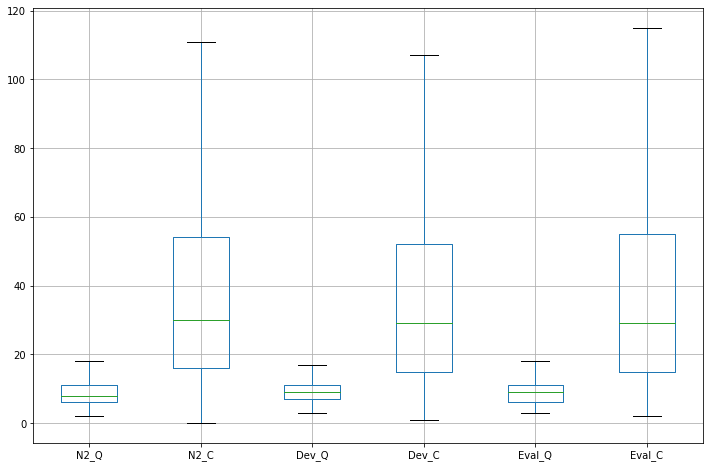
\includegraphics[width=1\textwidth]{figuras/cap-experimento/boxplot_number_of_words.png}
\caption{Diagrama de caixa para visualizar graficamente a distribuição da quantidade de palavras das questões e trechos de código-fonte por meio de quartis. Este diagrama de caixa exibe o Q1 (primeiro quartil), Q2 (segundo quartil) e Q3 (terceiro quartil). Eles referem-se aos percentis 25\%, 50\% e 75\% da Tabela~\ref{table:statistical-descriptive-of-pythons-sample}. O segundo quartil (Q2) refere-se a mediana. }. 
\label{fig:boxplot-number-of-words}
\end{figure}

\section{Treinamento}
\label{sec:treinamento}

Adotamos o mesmo procedimento de treinamento proposto por \cite{iyer-etal-2016-summarizing}. Utilizamos o conjunto $N_{2}$ composto por $60.083$ pares de questões e trechos de código-fonte. Durante o treinamento, do total de $60.083$ amostras, $42.058$ foram utilizadas para o conjunto de treinamento e $18.025$ para o conjunto de validação. Para escolha do modelo e avaliação final, foi utilizado o conjunto $N_{3}$ de dados anotados manualmente. A divisão das amostras para treinamento e avaliação podem ser visualizadas na Tabela~\ref{table:divisao-amostras}. 

O procedimento de treinamento utilizado foi: O modelo é treinado durante 500 épocas. Caso o valor da função de perda \textit{hinge} na amostra de treinamento fique abaixo de $0,0001$ ou o valor da função de perda na amostra de validação não diminua após 25 épocas, o treinamento é interrompido. A cada época, o modelo é avaliado na amostra \emph{DEV}. O intuito desta avaliação é obter o melhor modelo conforme a métrica \acrshort{mrr}. A ilustração deste procedimento pode ser visualizado na Figura~\ref{fig:evaluation-process}.

\begin{figure}[p]
\centering
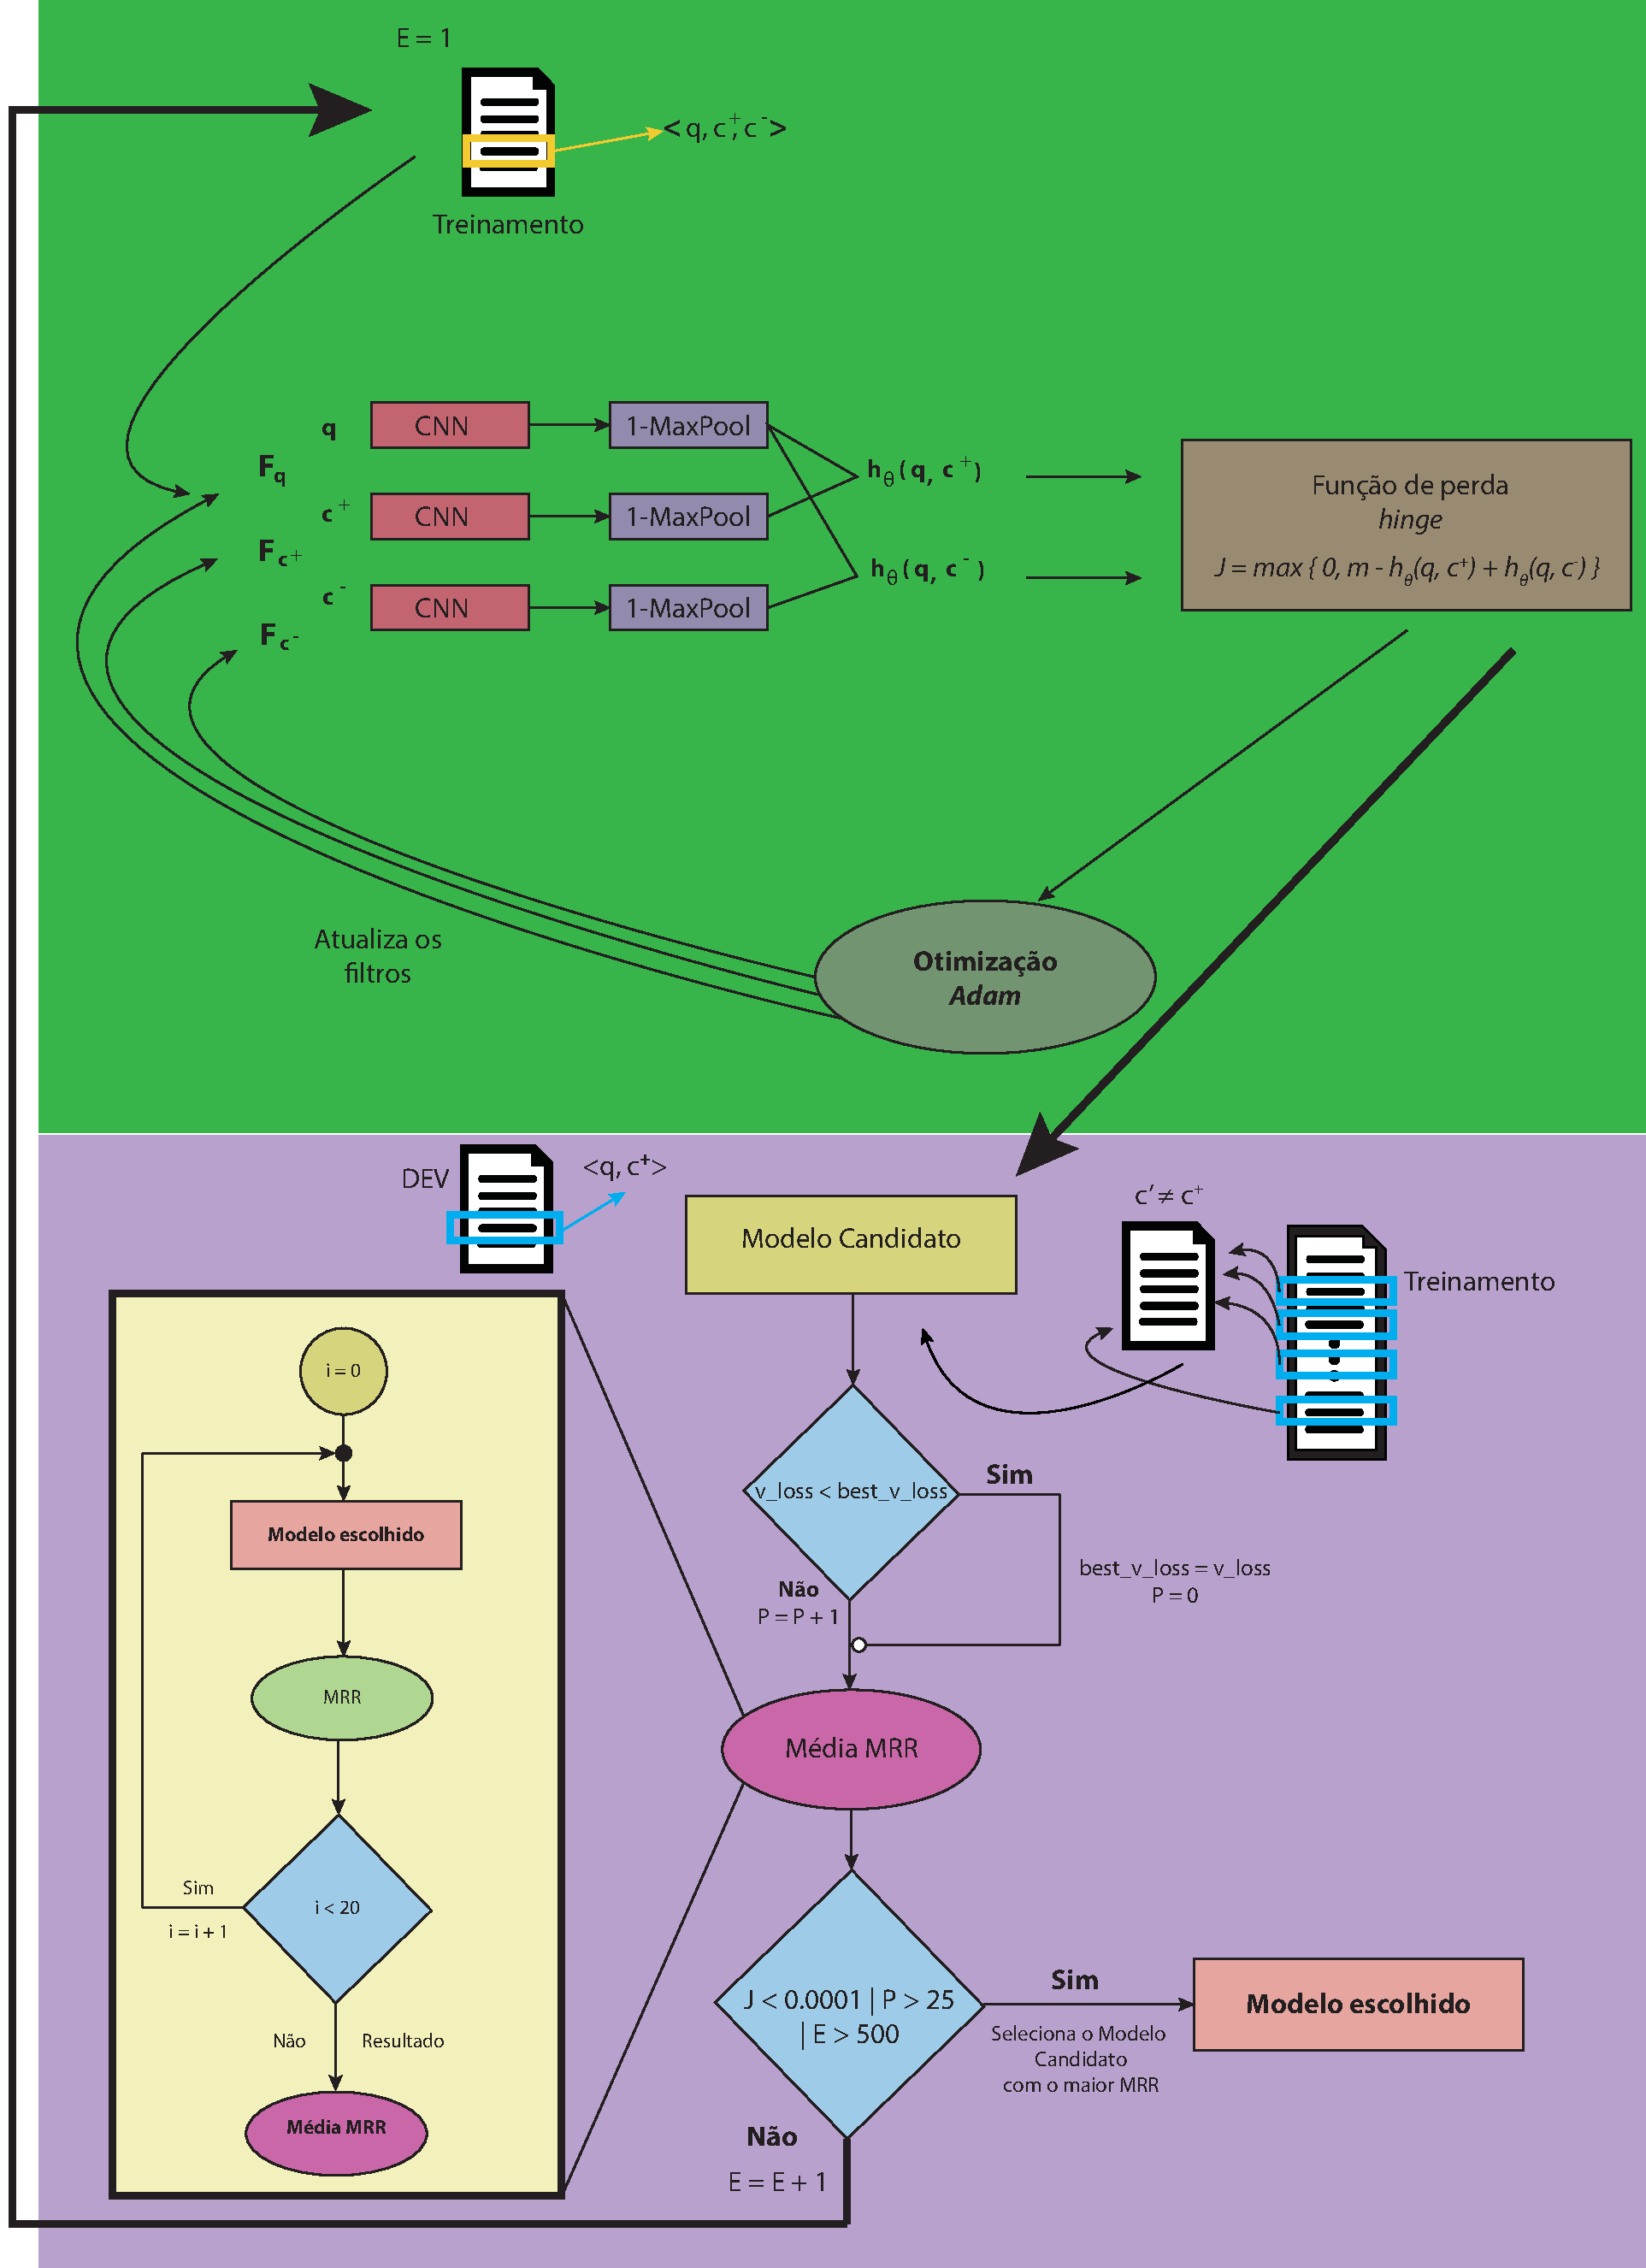
\includegraphics[height=1.3\textwidth]{figuras/cap-experimento/evaluation_process.pdf}
\caption{Ilustração do exemplo de treinamento de uma rede convolucional. Este procedimento é o mesmo adotado por \cite{iyer-etal-2016-summarizing}. $E$ é uma variável de controle para armazenar a quantidade de épocas. $P$ refere-se a quantidade de iterações seguidas em que não há diminuição do resultado da função de perda na amostra de validação. Os vetores de entrada dos modelos durante o treinamento são os vetores de representação distribuída $q, c^{+}, c^{'} \in \mathbb{R}^{150 X d}$, onde $150$ é o tamanho fixo dos vetores e $d$ é a dimensão do vetor. $F \in \mathbb{R}^{k X d}$ é o filtro convolucional, onde $k$ é o tamanho da janela e $d$ a dimensão do vetor. $h_{\theta}$ é a função \textit{cosine} de similaridade, $J$ é a função de perda \textit{hinge} e $m$ é a margem. O procedimento de treinamento está descrito na seção~\ref{sec:treinamento}.}
\label{fig:evaluation-process}
\end{figure}

Para cada par $<q_{i}, c_{i}^{+}>$ da amostra \emph{DEV}, onde $q_{i}$ uma questão e $c_{i}^{+}$ uma questão anotada como correta. Outros 49 distratores $c'$ são selecionados aleatoriamente da amostra de treinamento, tal que $c_{i}^{+} \neq c'$. Para cada questão, o modelo calcula a similaridade entre a questão e os trechos de código-fonte. O cálculo de similaridade é feito através da função $h_{\theta}$, onde $h_{\theta}$ é a função \textit{cosine}. 

Posteriormente, os trechos de código-fonte são ordenados de forma decrescente, do mais similar (maior pontuação) ao menos similar (menor pontuação). Com os trechos ordenados, obtém-se a posição do trecho $c_{i}^{+}$ para cálculo do \textit{reciprocal rank}. \textit{Reciprocal rank} é o inverso da posição da primeira ocorrência de $c_{i}^{+}$ encontrada no resultado. Com o \textit{reciprocal rank}, calcula-se o \acrshort{mrr}. \acrshort{mrr} é a média do \textit{reciprocal rank} para a amostra inteira \citep{Gu-deep-code-search:2018}:

\begin{equation}\label{eq:mrr}
MRR = \frac{1}{n} * \sum_{i = 1}^{n}\frac{1}{p_{i}^{+}}    
\end{equation}

Onde $n$ é a quantidade de questões presentes na amostra, $p_{i}^{+}$ é a posição da primeira ocorrência do trecho $c_{i}^{+}$ entre os trechos ordenados. 

Este procedimento é repetido durante 20 iterações. A cada iteração, outros 49 distratores são selecionados e, ao final, obtém-se a média \emph{MRR} do modelo. Basicamente, a cada época verificamos o resultado MRR do modelo comparando a resposta anotada como correta com outros 49 distratores. E selecionamos o modelo que obtiver a melhor média MRR. Este modelo escolhido será utilizado na avaliação final.

\section{Avaliação}
\label{sec:avaliacao}

A avaliação final na amostra \emph{EVAL} utiliza o mesmo procedimento da amostra \emph{DEV} descrito anteriormente. Quer dizer, calculamos o MRR para cada par $<q_{i}, c_{i}^{+}>$ da amostra \emph{EVAL} juntamente com outros 49 distratores $c'$ que são selecionados aleatoriamente da amostra de treinamento, tal que $c_{i}^{+} \neq c'$. Este procedimento de cálculo do MRR é repetido durante 20 iterações. Após as 20 iterações, obtemos a média final do nosso modelo. A ilustração deste procedimento pode ser visualizada na Figura~\ref{fig:final-evaluation-process}.

\begin{figure}[h]
\centering
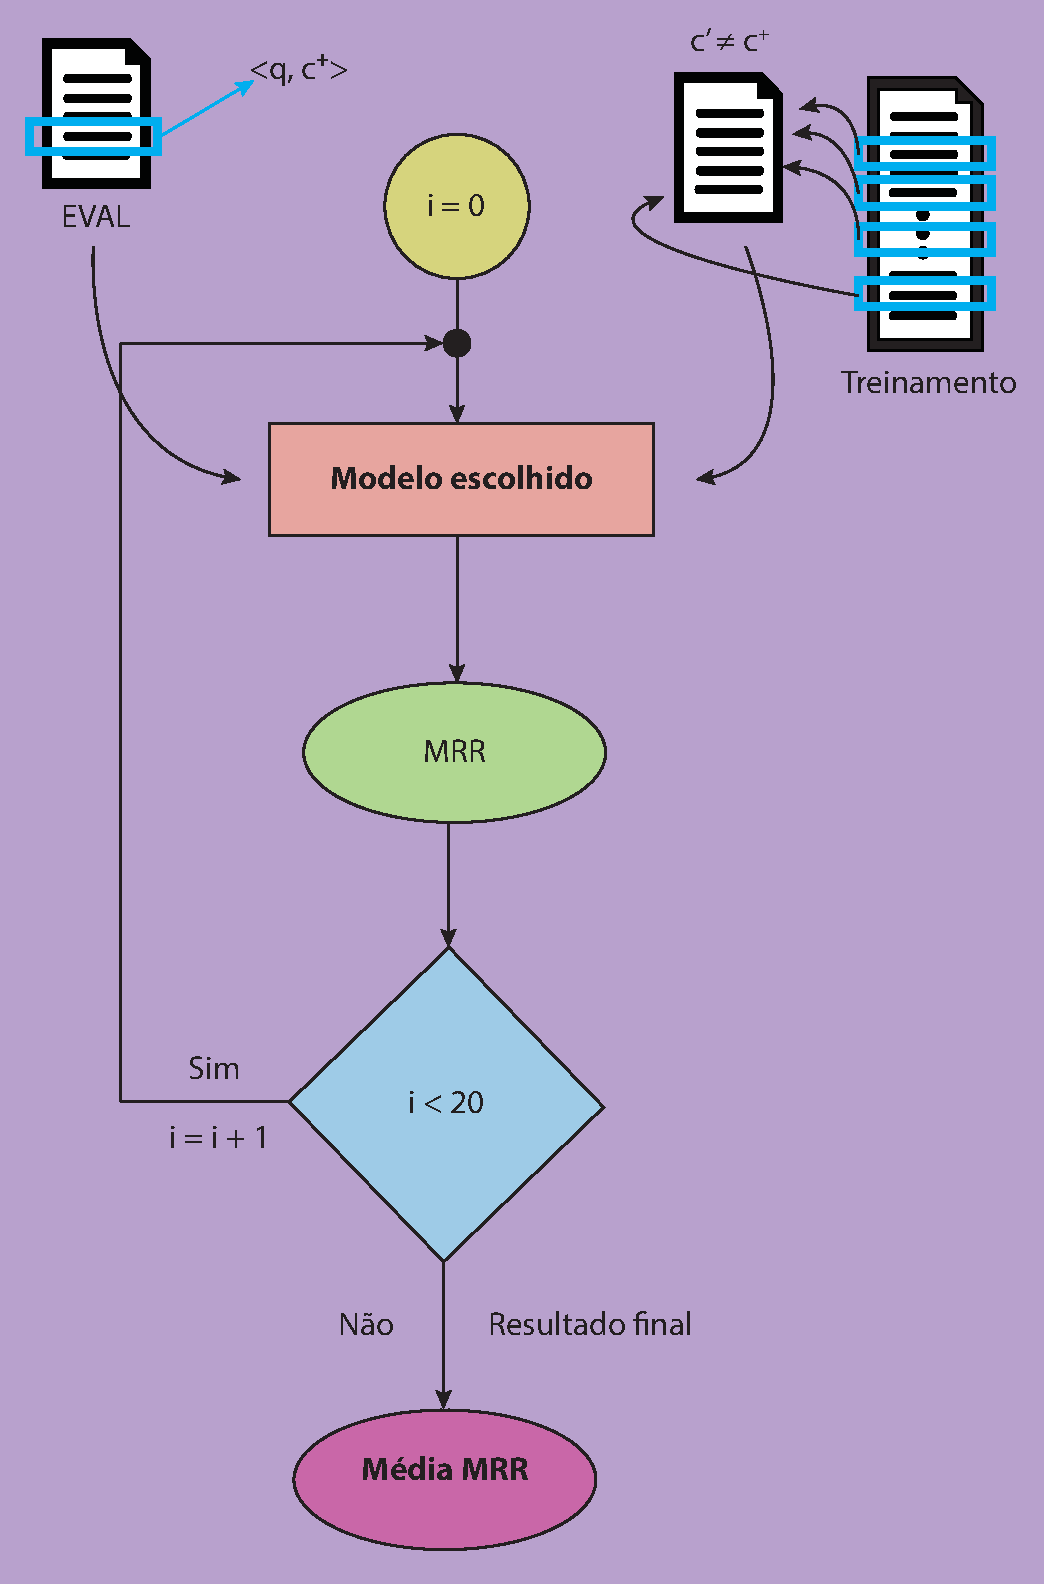
\includegraphics[height=1\textwidth]{figuras/cap-experimento/final_evaluation_process.pdf}
\caption{Ilustração do procedimento de avaliação proposto por \cite{iyer-etal-2016-summarizing}. O modelo com a maior média MRR no treinamento é avaliado na amostra EVAL. Durante 20 iterações, calculamos o MRR para os pares $<q, c^{+}>$ junto com outros 49 $c^{'}$ distratores, que são escolhidos da amostra de treinamento. Onde $q, c^{+}, c^{'} \in \mathbb{R}^{150 X d}$, tal $c^{+} \neq c^{'}$. A cada iteração outros 49 distratores $c^{'}$ são escolhidos. E ao final, obtemos o resultado do modelo.}
\label{fig:final-evaluation-process}
\end{figure}

\section{Pré-processamento}
\label{sec:pre-processamento}

Conforme o trabalho de \cite{tan-lstm-qa}, nós geramos uma matriz de representação distribuída $\bm{T_{v}}$ para o vocabulário das questões e para o vocabulário dos trechos de código-fonte, conforme citado no Capítulo~\ref{cap:abordagem}. Antes de gerar a matriz $\bm{T_{v}}$, utilizamos uma função disponibilizada por \cite{yao-2018} para fazer um pré-processamento dos trechos de código-fonte. Essa função substitui os valores literais numéricos e textos pelas palavras \emph{"NUMBER"} e \emph{"STRING"}. Além disso, os comentários são removidos e as variáveis são substituídas por \emph{"VAR"}. O caractere de quebra de linha é substituído por \emph{"NEWLINE"}.

A matriz $\bm{T_{v}}$ é gerada pelo \textit{word2vec} com \textit{skip-gram}. Na Figura~\ref{fig:tsne-code-snippet-python}, podemos visualizar um exemplo da representação do vetor de representação distribuída gerada pelo \textit{word2vec}. Essa imagem foi criada com o auxílio da ferramenta \textit{t-SNE}. Ela auxilia na visualização de dados de dimensão elevada \citep{scikit-learn-tsne-2019, quora-tsne-2019}. De acordo com a Figura~\ref{fig:tsne-code-snippet-python}, as palavras \emph{file}, \emph{open}  e \emph{write} são similares. Assim como \emph{set}, \emph{dict} e \emph{list}, por exemplo.

\begin{figure}[h]
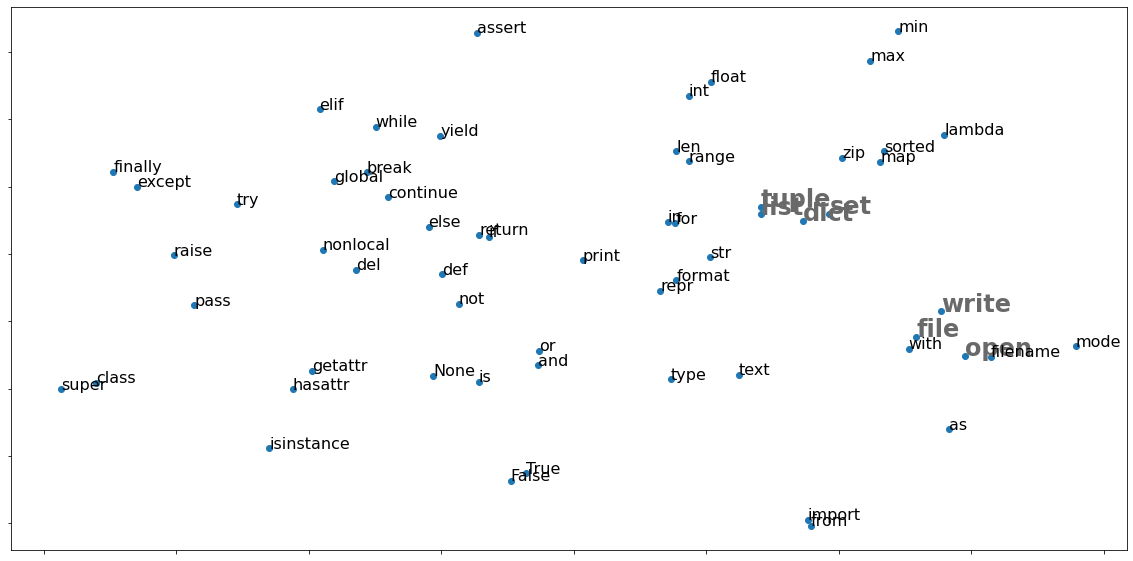
\includegraphics[width=1\textwidth]{figuras/cap-experimento/code_tsne.png}
\caption{Representação em 2D do vetor de representação distribuída de trechos de código-fonte. Imagem gerada através da ferramenta t-SNE. O vetor de representação distribuída foi criado a partir da amostra de pares de questões e trechos de código-fonte em Python disponibilizada por \cite{yao-2018}. Vetor criado utilizando o \textit{word2vec} com o algoritmo \textit{skip-gram} e o parâmetro \textit{window} com o valor $5$.}
\label{fig:tsne-code-snippet-python}
\end{figure}

\section{Arquiteturas}

Para este estudo, comparamos a arquitetura CNN com outras duas arquiteturas: \textit{Unif} e \textit{Embedding}. A arquitetura \textit{Unif} proposta por \cite{cambronero-deep-learning-code-search:2019} utiliza duas abordagens diferentes para representação das questões e trechos de código-fonte. No caso das questões, os vetores de representação distribuída de cada palavra são combinados através de uma média aritmética simples. Quanto aos trechos de código, aplica-se o \gls{mecanismo-atencao} que calcula uma média ponderada sobre os vetores de representação distribuída e aprende a ``prestar atenção`` nas palavras mais importantes.  Já a arquitetura \textit{Embedding} combina os vetores de representação distribuída de cada palavra através de uma camada \textit{max pool}. As figuras~\ref{fig:cnn-architecture}, \ref{fig:unif-architecture} e \ref{fig:embedding-architecture} ilustram as arquiteturas utilizadas.
\begin{figure}[h]
    \centering
    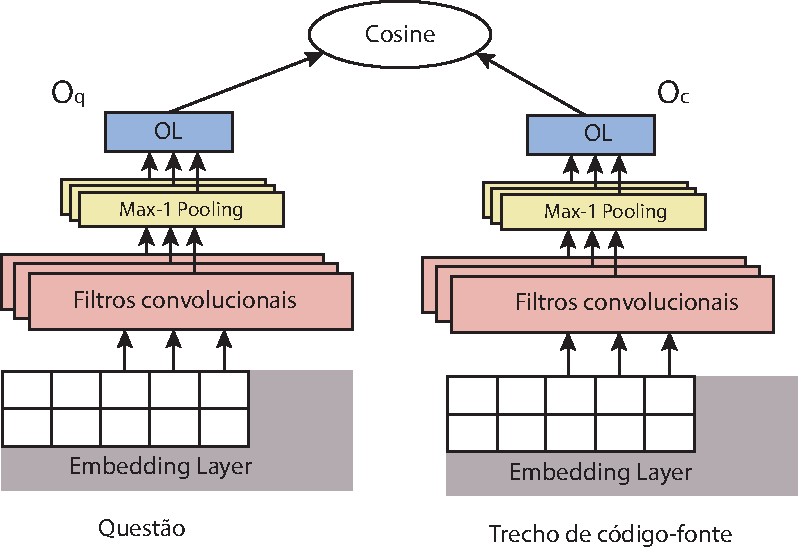
\includegraphics[width=0.8\textwidth]{figuras/cap-experimento/cnn-architecture-proposal.pdf}
    \caption{Figura da arquitetura CNN descrita no Capítulo~\ref{cap:abordagem}. O termo \emph{Embedding Layer} refere-se a camada composta por vetores de representação distribuída. OL é o acrônimo de \emph{Output Layer}, i.e., camada de saída. $O_{q}$ e $O_{c}$ indicam a saída do vetor de representação final das questões e trechos de código-fonte, respectivamente. \emph{Cosine} indica a função de similaridade.}
    \label{fig:cnn-architecture}
\end{figure}

\begin{figure}[h]
    \centering
    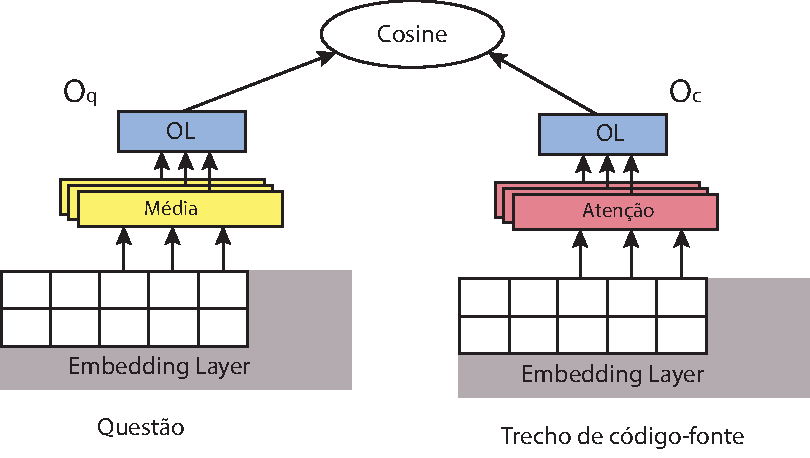
\includegraphics[width=0.8\textwidth]{figuras/cap-experimento/unif-architecture.pdf}
    \caption{Figura da arquitetura \Gls{unif} proposta por \cite{cambronero-deep-learning-code-search:2019}. \emph{Embedding} refere-se a camada composta pelos vetores de representação distribuída. \emph{Média} é camada que combina os vetores através de uma média aritmética simples. \emph{Atenção} refere-se ao \gls{mecanismo-atencao}, que combina os vetores através de uma média ponderada e aprende a ''prestar atenção'' nos termos mais relevantes. \emph{OL} é o acrônimo de \emph{Output Layer}, i.e., camada de saída. $O_{q}$ e $O_{c}$ referem-se ao vetor de representação final das questões e trechos de código, respectivamente. \emph{Cosine} indica a função de similaridade. }
    \label{fig:unif-architecture}
\end{figure}

\begin{figure}[h]
    \centering
    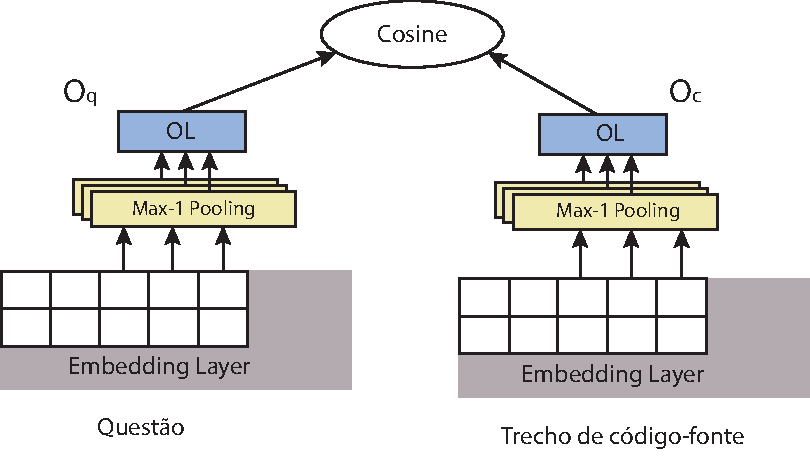
\includegraphics[width=0.8\textwidth]{figuras/cap-experimento/embedding-architecture.pdf}
    \caption{Figura da arquitetura de referência \textit{Embedding} para comparação. \emph{Embedding Layer} refere-se a camada composta pelos vetores de representação distribuída. \emph{OL} é o acrônimo de \emph{Output Layer}, i.e., camada de saída. $O_{q}$ e $O_{c}$ referem-se aos vetores de representação final das questões e trechos de código, respectivamente. \emph{Cosine} refere-se a função de similaridade. Figura utilizada no artigo \cite{marcelo-vem-2019}.}
    \label{fig:embedding-architecture}
\end{figure}
Nas figuras \ref{fig:cnn-architecture}, \ref{fig:unif-architecture} e \ref{fig:embedding-architecture}, a palavra \textit{Embedding Layer} refere-se ao vetor de representação distribuída das palavras. \emph{OL} é um acrônimo de \textit{Output Layer} ou camada de saída. $O_{q}$ indica a camada de saída da questão. $O_{c}$ indica a camada de saída do trecho de código-fonte. As arquiteturas CNN e \textit{Embedding} utilizam uma camada \textit{max pool}. E todas, ao final, calculam a similaridade atravás da função \textit{cosine}. Os ajustes dos hiper-parâmetros são discutidos com mais detalhes no Apêndicê~\ref{ape:ajuste-hiper-parametros-cnn} e no Capítulo~\ref{cap:resultados}, que também apresenta os resultados dos experimentos.

